\subsection{\bf Flow Size Analysis}
We have analyzed the flow size for each specific type of flows, and the results are shown in figure ~\ref{fig:read_size}, ~\ref{fig:write_size} and ~\ref{fig:replica_size}.



%\begin{comment}
%\begin{figure*}[htb]
%\begin{figure*}[!ht]
%\label{fig:read_size}
%\centering	
%   \begin{tabular}{@{}cc@{}}
%	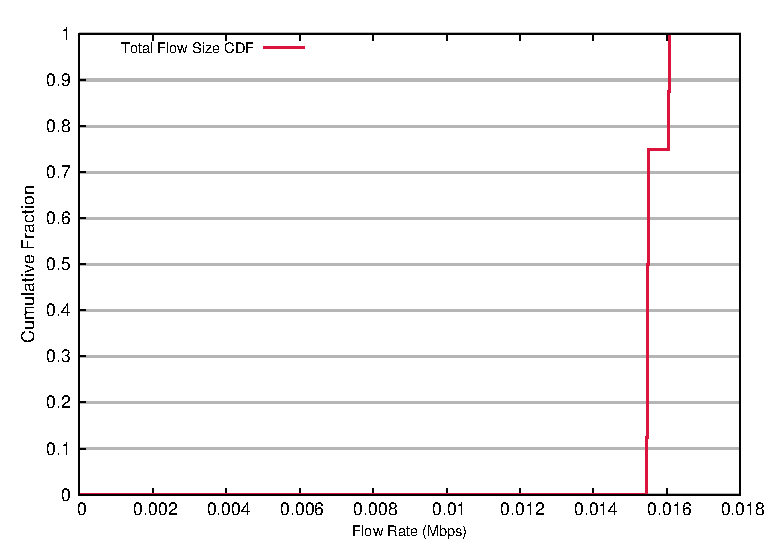
\includegraphics[width=.55\textwidth]{figures/4read/24_28_flow_size.eps} &
%	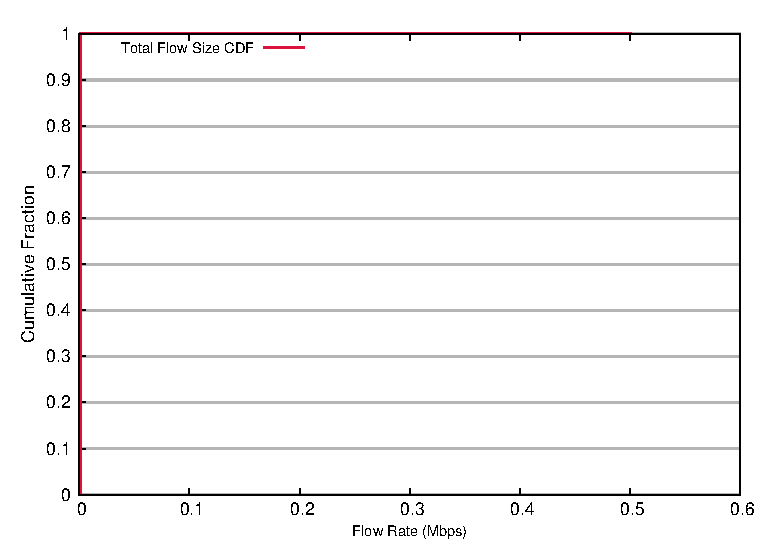
\includegraphics[width=.55\textwidth]{figures/4read/8_12_flow_size.eps}  \\
%	\multicolumn{2}{c}{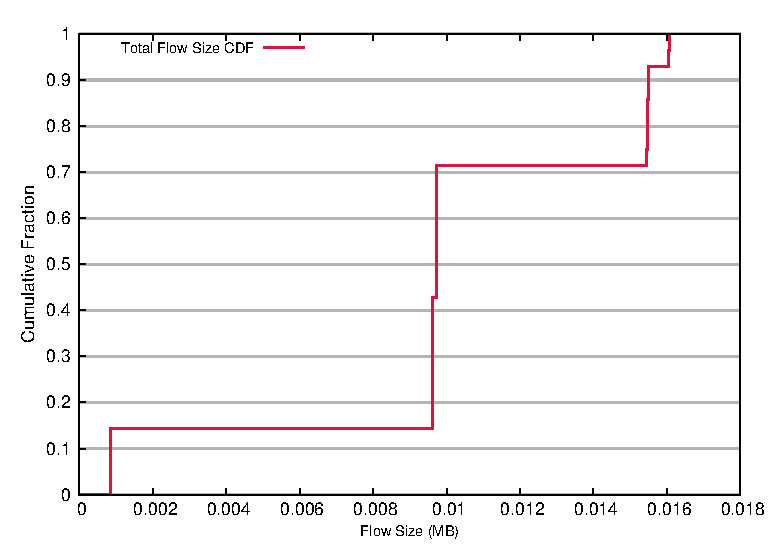
\includegraphics[width=.73\textwidth]{figures/4read/flow_size.eps}}
%    \end{tabular}
%\caption{Read Flow Size Distribution}
%\end{figure*}
%\end{comment}

%\begin{figure*}[!htpb]
\begin{figure*}
\centering
  \begin{subfigure}[b]{.45\linewidth}
   \centering
	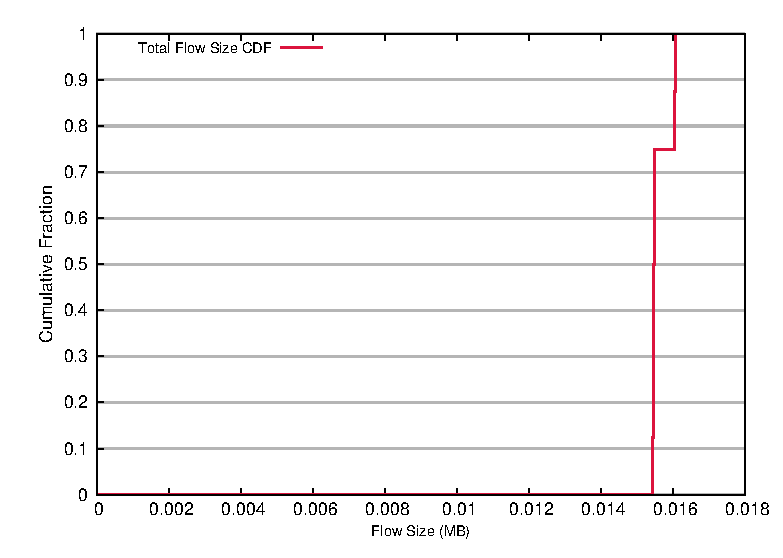
\includegraphics[width=.99\textwidth]{figures/4read/24_28_type_size.eps} 
	\caption{RPC between Client and DataNodes}\label{fig:read_size:rpc}
   \end{subfigure}%
  \begin{subfigure}[b]{.45\linewidth}
   \centering
	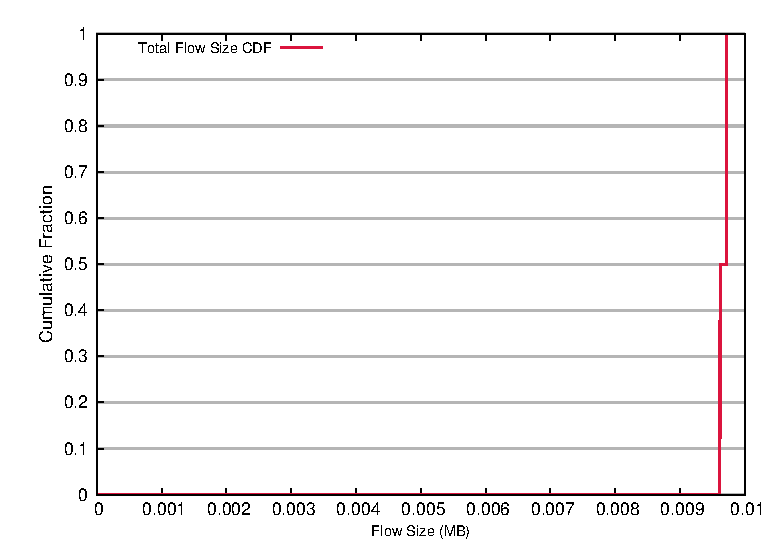
\includegraphics[width=.99\textwidth]{figures/4read/24_28_20_16_type_size.eps} 
	\caption{Should have read data transfer here}\label{fig:read_size:nn_rpc}
   \end{subfigure} \\%
  \begin{subfigure}[b]{.55\linewidth}
   \centering
	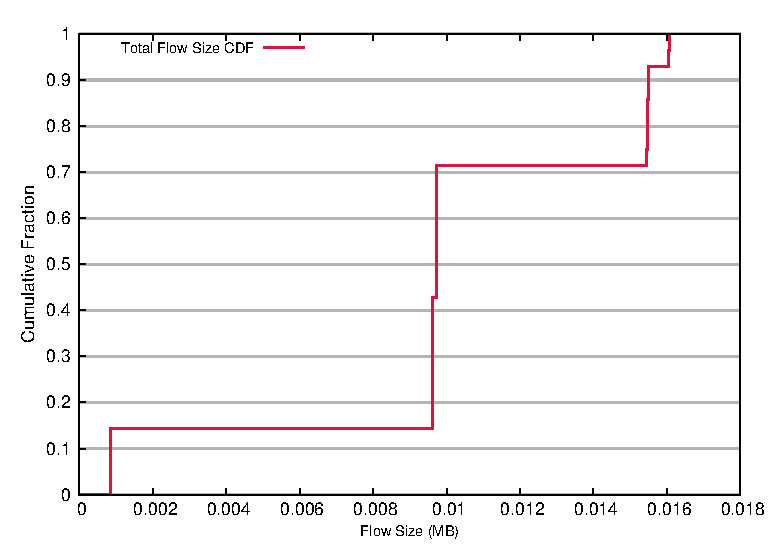
\includegraphics[width=.99\textwidth]{figures/4read/flow_size.eps}
	\caption{All Traffic}\label{fig:read_size:all}
   \end{subfigure}%
\caption{Read Flow Size Distribution}
\label{fig:read_size}
\end{figure*}

From figure \ref{fig:read_size} we could see that for the read workload, all the flows transfer very little data. They are mainly used for RPC calls/responses to transfer control messages. This means that HDFS served all the read locally without using the network. Because HDFS is carefully tuned to place data locally, and serve requests from local nodes whenever possible, this result is expected and actually shows that HDFS does a good job in terms of data locality.

\begin{figure*}[!htpb]
\centering
  \begin{subfigure}[b]{.45\linewidth}
   \centering
	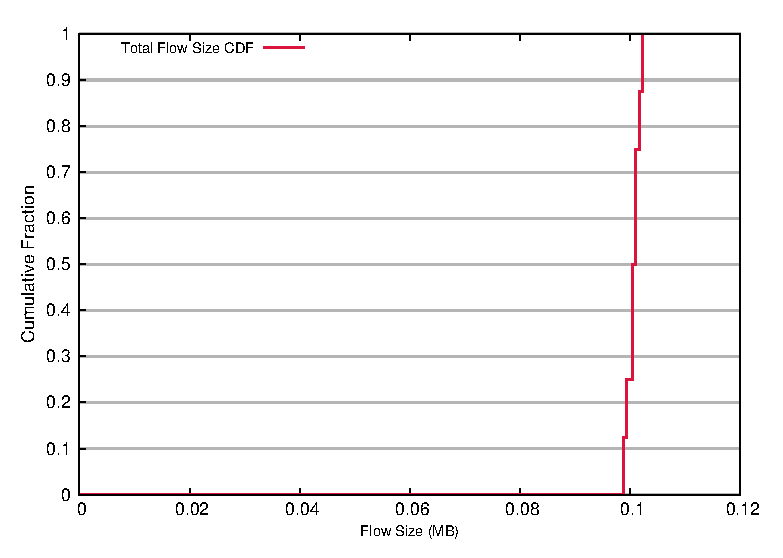
\includegraphics[width=.99\textwidth]{figures/6writes/24_28_type_flow_size.eps} 
	\caption{DataNodes RPC with NameNode}\label{fig:write_size:dn_rpc}
   \end{subfigure}%
  \begin{subfigure}[b]{.45\linewidth}
   \centering
	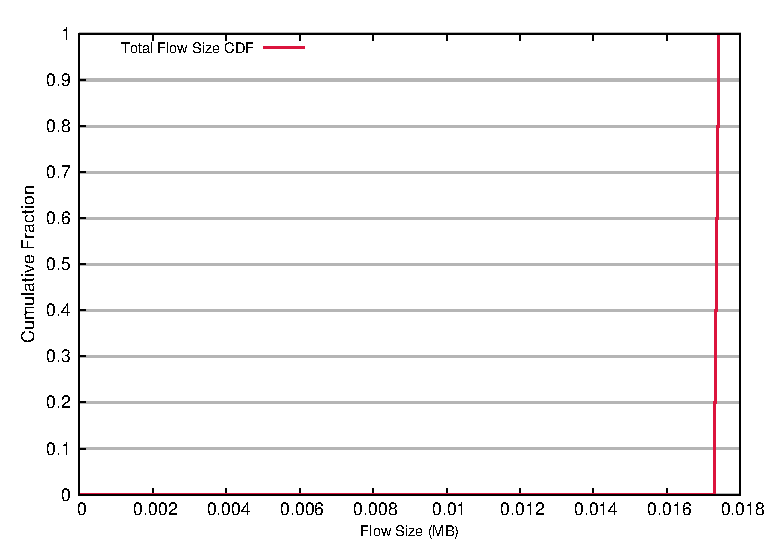
\includegraphics[width=.99\textwidth]{figures/6writes/24_28_20_16_type_flow_size.eps} 
	\caption{Client and DataNodes RPC with NameNode}\label{fig:write_size:dc_rpc}
   \end{subfigure} \\%
  \begin{subfigure}[b]{.45\linewidth}
   \centering
	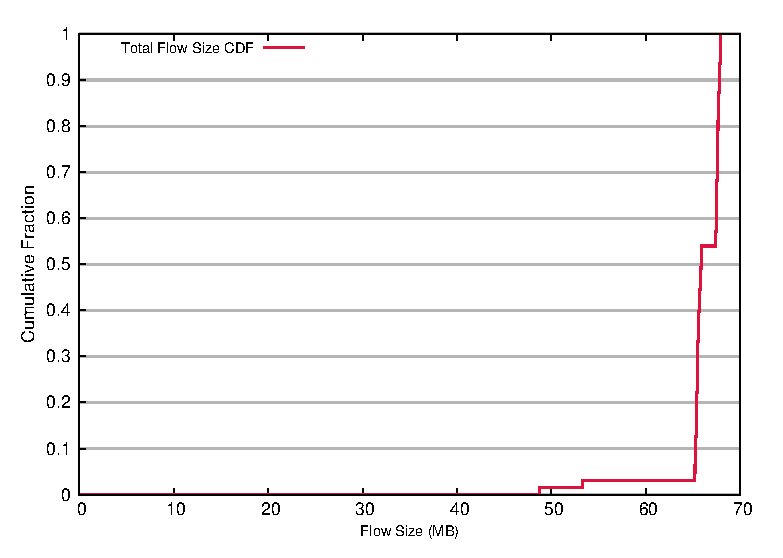
\includegraphics[width=.99\textwidth]{figures/6writes/36_44_type_flow_size.eps} 
	\caption{Pipelined Writes between DataNodes}\label{fig:write_size:pipe_write}
   \end{subfigure} %
  \begin{subfigure}[b]{.45\linewidth}
   \centering
	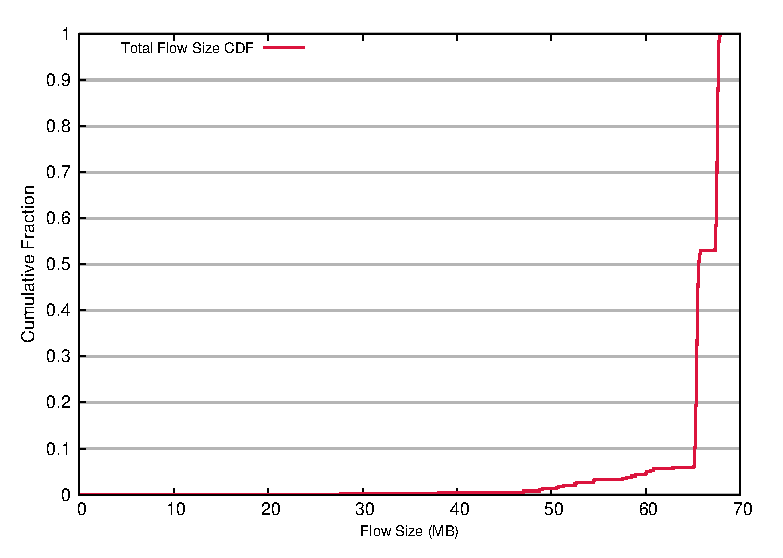
\includegraphics[width=.99\textwidth]{figures/6writes/32_36_type_flow_size.eps} 
	\caption{Client Data Transfer to DataNodes}\label{fig:write_size:client_write}
   \end{subfigure} \\%
  \begin{subfigure}[b]{.55\linewidth}
   \centering
	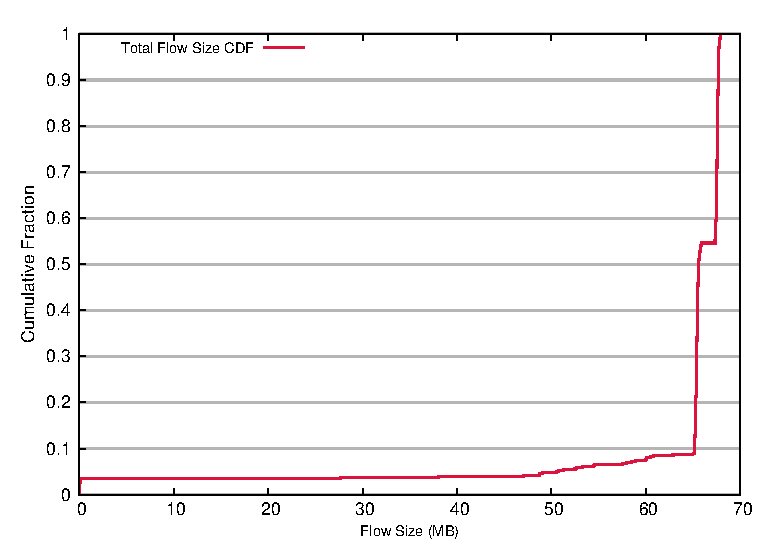
\includegraphics[width=.99\textwidth]{figures/6writes/flow_size.eps}
	\caption{All Traffic}\label{fig:write_size:all}
   \end{subfigure}%
\caption{Write Flow Size Distribution}
\label{fig:write_size}
\end{figure*}


The flow size distribution of the write workload shown in figure ~\ref{fig:write_size} revealed some information about HDFS's internal operation. We can see that there are two kinds of flows, RPC flows, which typically has very small data transferred; and data transfer flows, including the pipelined data transfer between data nodes and the data client writes to the data nodes, which is around 65 MB. This is in compliance with the fact that HDFS has separate flows for RPC calls/responses and data transfers; and data transfer is done in the unit of blocks, which is 64 MB in our configuration. We could also see that less than 5\% of the flows are used for RPC calls to transfer control information, while the majority of the flows are used for data transfer, which is as expected. 

\begin{figure*}[!htpb]
\centering
  \begin{subfigure}[b]{.45\linewidth}
   \centering
	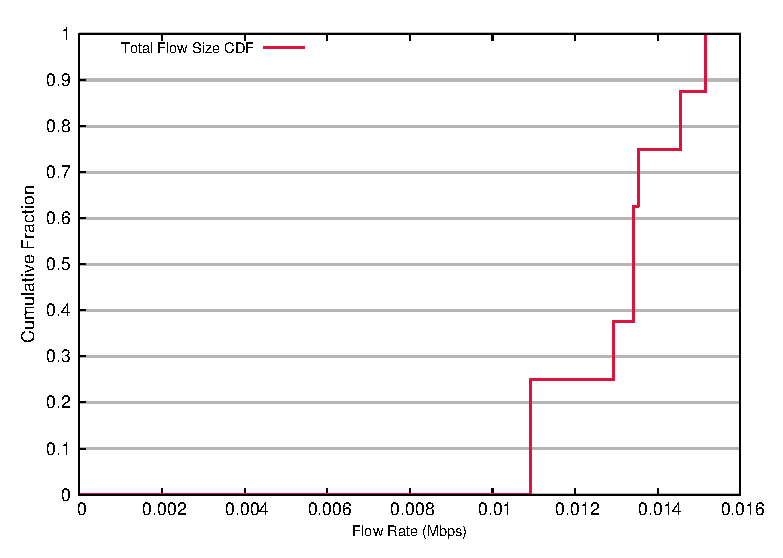
\includegraphics[width=.99\textwidth]{figures/replica_change/24_28_flow_size.eps} 
	\caption{DataNodes RPC with NameNode}\label{fig:replica_size:rpc}
   \end{subfigure}%
  \begin{subfigure}[b]{.45\linewidth}
   \centering
	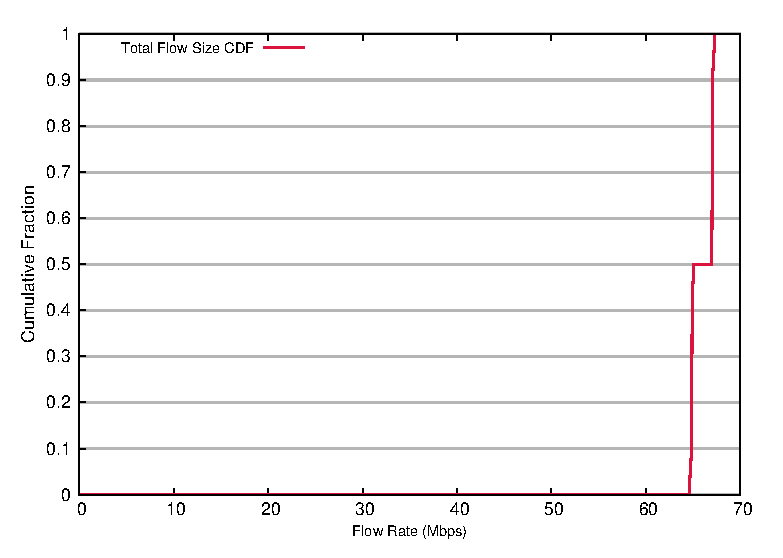
\includegraphics[width=.99\textwidth]{figures/replica_change/36_32_flow_size.eps} 
	\caption{Pipelined Writes between DataNodes}\label{fig:replica_size:pipe_write}
   \end{subfigure} \\%
  \begin{subfigure}[b]{.55\linewidth}
   \centering
	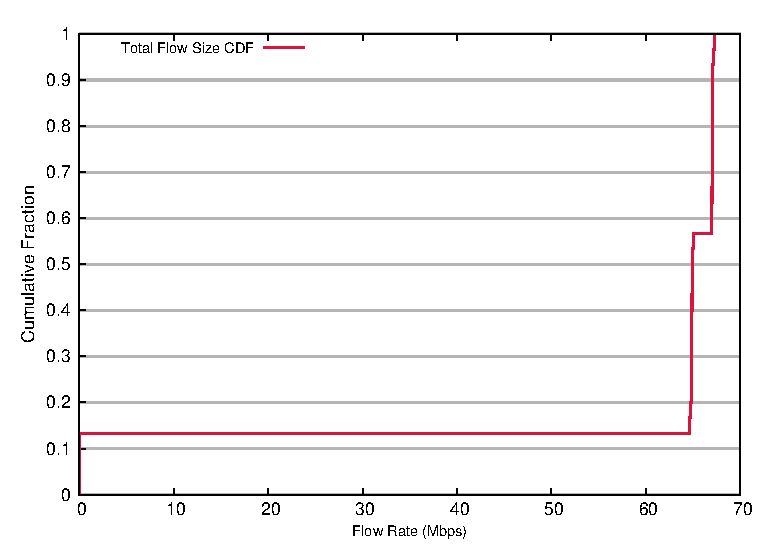
\includegraphics[width=.99\textwidth]{figures/replica_change/flow_size.eps}
	\caption{All Traffic}\label{fig:read_size:all}
   \end{subfigure}%
\caption{Replciation Level Change Flow Size Distribution}
\label{fig:replica_size}
\end{figure*}

The flow size distribution of the replication level change workload in figure ~\ref{fig:replica_size} exhibited the same characteristics, except for that we have less data transfers and relatively more control messages. 

